% !TEX encoding = UTF-8 Unicode
% \documentclass{article}
% \usepackage{../../superstyle}
% \usepackage{listings}
% \usepackage{amsmath}
% \begin{document}
% remove all before

%oppgavetekst
Plot the solution from Step 1 against the correct solution
\begin{align}
	y(x) = (f/24EI)x^2(x^2 − 4Lx + 6L^2)
\end{align}
where f = f(x) is the constant defined above.
\newline
\newline
Check the error at the end of the beam, x = L meters. In this simple case the derivative approximations are exact, so your error should be near machine roundoff.


\vspace{5mm}
Løsning

\begin{lstlisting}[caption={oppgave2.m}]
%definerer steglengden
tall1 = lagmatrise(10)\konstantkrefter(10);
tall2 = korrektutregning(10);

format long
%skriver ut forskjellen mellom slutten av planken for de 2 forskjellige
%utregningene
disp(tall1(10)-tall2(10));

%lager x-verdier til grafen
x = (1:10)/5;

%lager graf med x som 
%plot(x, [tall1, tall2]);
%plot(x, tall2); 
plot(x, tall1, x, tall2); 
\end{lstlisting}

% \noindent der konstante krefter er definert slik:

\begin{lstlisting}[caption={konstantkrefter.m}]
function [B] = konstantkrefter(n)

%lager h?yresiden av matriseligningen. (h^4/EI) * f(x) 
%deler opp bjelken i n lengder med lengde h 
h = 2 / n;        

%regner ut kraften f(x) 
kraft = -9.81*480*0.3*0.03; 

%definerer E og I som gitt i oppgaven
E = 1.3*10.^(10); 
I = (0.3*0.03.^3)/12; 

%lager en n h?y matrise, bredde 1, av enere, som ganges med kraft og h^4/EI.
B = ones(n, 1) * h^4/(E*I) * kraft;

\end{lstlisting}

\vspace{3mm}
\noindent Dette gir denne grafen\\

% \includegraphics[scale=0.35]{errorplot2}

\begin{figure}[h]
    \centering
    \includegraphics[width=0.8\textwidth]{sections/Exercise2/errorplot2}
    % \includegraphics[width=0.8\textwidth]{errorplot2}
    \caption{Error plot}
    \label{fig:errorplot2}
\end{figure}
 
som man kan se i figur \ref{fig:errorplot2}, er de to linjene veldig nerme hverandre.


% remove after
% \end{document}